\begin{figure}
\begin{tabular}{@{}c@{}c@{}}
\begin{subfigure}[b]{0.45\textwidth}
\begin{center}
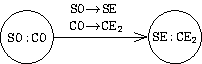
\includegraphics[scale=1.35]{chapters/figures/figIsEmptyProductCfg.pdf}
\end{center}
\vspace{6.5px}
\caption{\label{fig:isemptyproductcfg}Product-CFG between \cref{fig:isemptyspeccfg,fig:isemptyccfg}}
\end{subfigure}%
&
\begin{subfigure}[b]{0.55\textwidth}
\begin{center}
\begin{footnotesize}
\begin{tabular}{cl}
\toprule
{\bf PC-Pair} & \multicolumn{1}{c}{\bf Invariants} \\
\toprule
(\scpc{0}{0}) & $\circled{P}\  \sv{s} \indEq{} \lifted{str}{\mem{}}{u8[]}{\cv{s}}$ \\
\midrule
(\scpc{E}{E_2}) & $\circled{E} \  \sv{ret} = \cv{ret}$ \\
\bottomrule
\end{tabular}
\end{footnotesize}
\end{center}
\caption{\label{fig:isemptyinvs}Invariants table for product-CFG in \cref{fig:isemptyproductcfg}}
\end{subfigure}%
\\
\end{tabular}
\caption{\label{fig:isemptyproductcfgandinvs}Product-CFG and its associated node invariants for CFGs in \cref{fig:isemptyspeccfg,fig:isemptyccfg}.}
\end{figure}
